\documentclass[../../main.tex]{subfiles}

\begin{document}
        Für einen theoretischen LC Schwingkreis gilt mit der Induktivität $L$ und der Kapazität $C$ die Resonanzfrequenzbeziehung $f(L,C) = 1/\sqrt{L\cdot C}$. In dem Messaufbau unseres Versuchs ist die Kapazität $C$ durch einen variablen Hardwarekondensator variierbar. Bei fester, jedoch zuerst unbekannter Induktivität $L$ können wir unter der Annahme einer Startverschiebung $C_0$ die Resonanzfrequenz $f_L$ und die Induktivität $L$ des Schwingkreises durch eine Kurvenanpassung der Form 
        \begin{align}
            f(C + C_0,L) = \frac{1}{\sqrt{L\cdot (C + C_0)}}
        \end{align}
        bestimmen \cite[ch 1.4.3]{doc:EFNMRStudentManual}. Die Wahl von $C_0$ als einzigen Variationsparameter neben $L$ stellt sich kurvenanpassungstechnisch als ausreichend heraus, da mit $L$ bereits eine Skalierung von $C + C_0$ vorliegt und $a=1$ in der allgemeinen Kurvenanpassung $f(x) = a / \sqrt{b\cdot (x + x_0)}$ gemäß der Resonanzfrequenzformel $f(L,C)$ gesetzt werden kann.
        Für die spätere Bestimmung von $C_{opt}$ durch Kenntnis von $L$ und $f_L$ invertieren wir $C\mapsto f(C + C_0)$ und erhalten 
        \begin{align}
            C_{opt}(f,L,C_0) = \frac{1}{f^2\cdot L} - C_0. \label{eq:4:Capacitance}
        \end{align}
        Eine Kurvenanpassung der Datenwerte liefert uns zunächst die in Tabelle \ref{tab:4:LCRResonance} aufgeführten Parameter. Optisch erhalten wir eine sehr gute Übereinstimmung zwischen Theorie und Messwerten, wie in Abbildung \ref{fig:4:LCRResonance} zu sehen ist.
        \begin{table}[H]
            \centering
            \begin{tabular}{c|ll|ll}
                 \textbf{Durchgang} & $L$ in $\si{\henry}$ & $u(L)$ in $\si{\henry}$ & $C_0$ in $\si{\nano\farad}$ & $u(C_0)$ in $\si{\nano\farad}$ \\
                \hline
                $1$ & $1.64\cdot 10^{-8}$ & $2.34\cdot 10^{-11}$ & $4.27$ & $0.02$ \\
                $2$ & $1.64\cdot 10^{-8}$ & $2.34\cdot 10^{-11}$ & $4.27$ & $0.02$ \\
                \hline
                avg. & $1.64\cdot 10^{-8}$ & $3.31\cdot 10^{-11}$ & $4.27$ & $0.03$
            \end{tabular} 
            \caption{Parameterübersicht der Funktion $f(C,L)$ für die aufgenommenen Messwerte.}
            \label{tab:4:LCRResonance}
        \end{table}
        \begin{figure}[H]
            \centering
            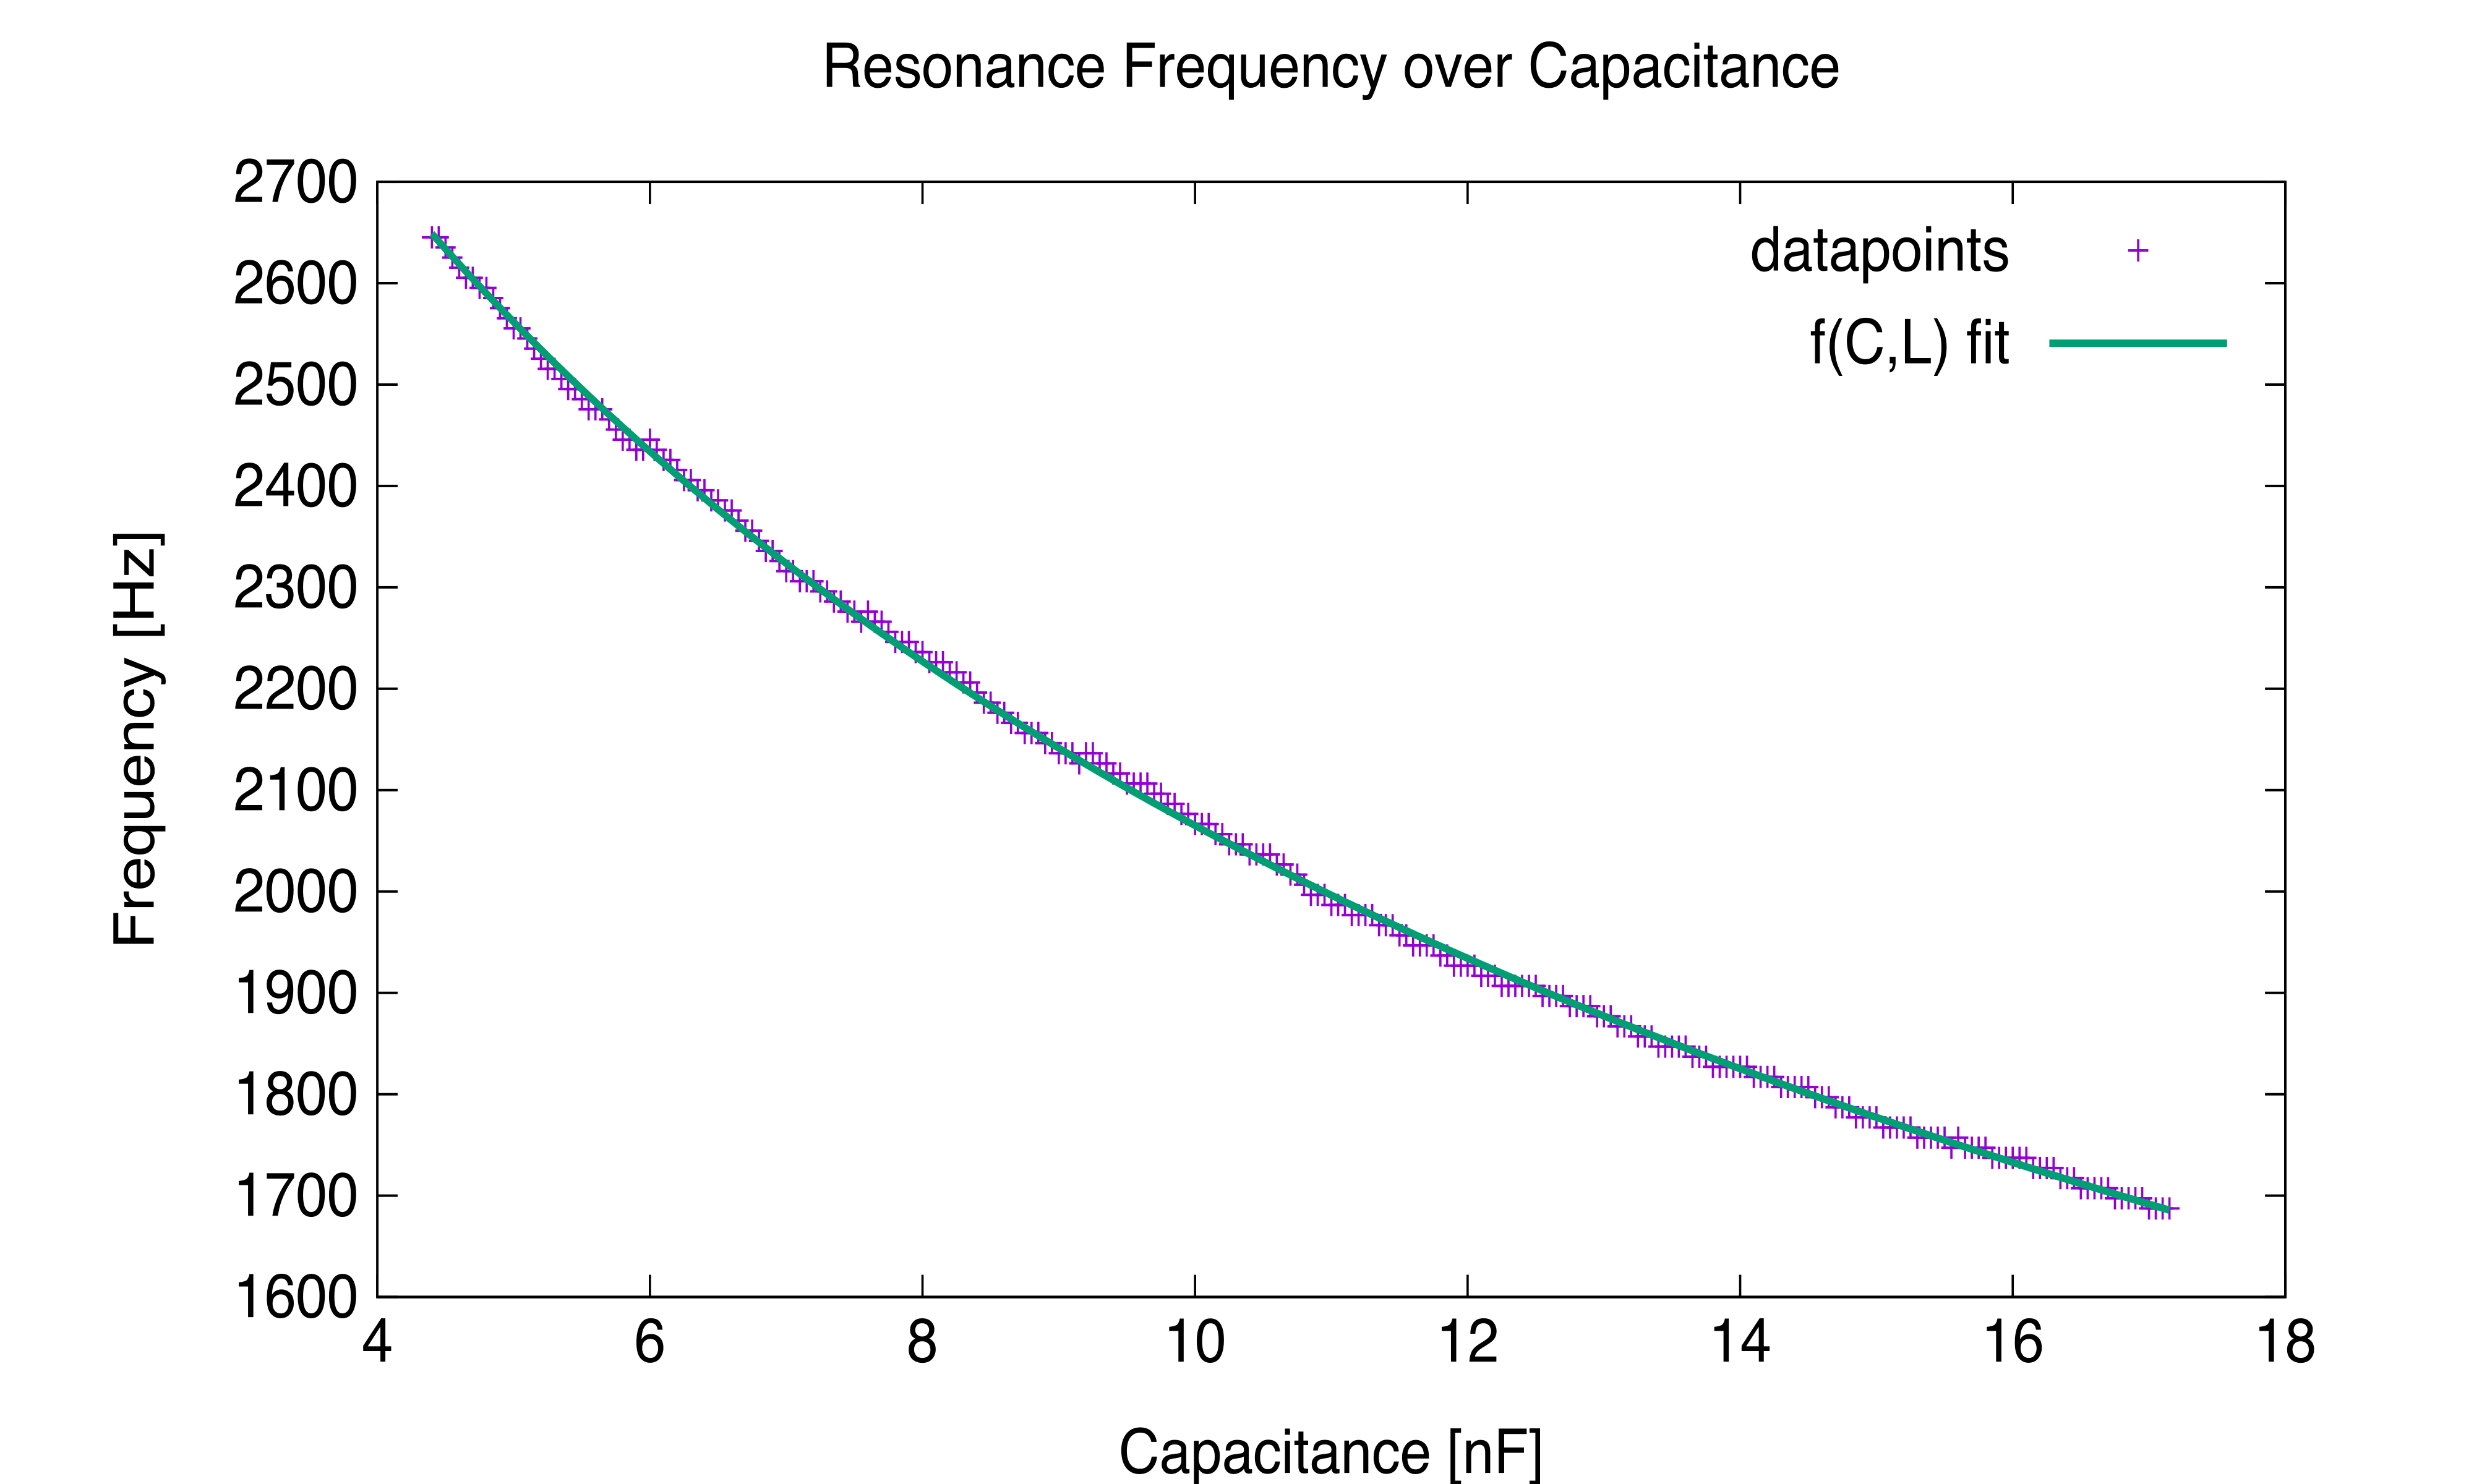
\includegraphics[width=11cm]{Bilddateien/4/Messung1_Resonance_Freq_vs_Capacitance.png}
            \caption{Messung der Resonanzfrequenz in Abhängigkeit der Kapazität am Beispiel des ersten Versuchdurchgangs.}
            \label{fig:4:LCRResonance}
        \end{figure}
        Die mittleren Unsicherheiten sind wieder mit gewöhnlicher Unsicherheitsfortpflanzung der Funktion plus bestimmt worden. Mithilfe der durch die Kurvenanpassung erhaltenen Parameter $L$ und $C_0$ können wir unter Hinzuzug der bereits in Kapitel \ref{subsec:2:InitialeMessung} bestimmten Larmorfrequenz $f_L$ die optimale Kondensatorkapazität $C_{opt}$ bestimmen. Diese ist durch Gleichung \eqref{eq:4:Capacitance} gegeben und bestimmt sich zu den Werten in Tabelle \ref{tab:4:OptimalCapacitance}.
        \begin{table}[H]
            \centering
            \begin{tabular}{c|cc}
                \hline
                 & $C_{opt}$ in $\si{\nano\farad}$ & $u(C_{opt})$ in $\si{\nano\farad}$ \\
                \hline\hline
                avg. & $10.92$ & $0.181$\\
                \hline
            \end{tabular}
            \caption{Optimale Kondensatorkapazität $C_{opt}$ für die beiden Durchgänge gemittelt.}
            \label{tab:4:OptimalCapacitance}
        \end{table}
        Dabei wurden zur Berechnung der Unsicherheit $u(C_{opt})$ die Unsicherheitsfortpflanzung der Funktion $C_{opt}$ und die Unsicherheiten der Parameter $L$ und $C_0$ verwendet. Es gilt dabei für $x:=(f,L,C_0)$ der Zusammenhang
        \[
            u(C_{opt})(x) := \sqrt{\bigl(\partial_1C_{opt}(x)\bigr)^2\cdot u(f)^2 + \bigl(\partial_2C_{opt}(x)\bigr)^2\cdot u(L)^2 + \bigl(\partial_3C_{opt}(x)\bigr)^2\cdot u(C_0)^2}.
        \]
        
    % \bibliography{../Literatur.bib}

\end{document}